\subsection{ISO/SAE 21434: Overview}\label{subsec:iso-sae-21434}

Released in August 2021, the ISO/SAE 21434 standard is a joint standard
developed by the \href{https://www.iso.org/home.html}{International Organization for Standardization (ISO)} and the
\href{https://www.sae.org/}{Society of Automotive Engineers (SAE)} to address the cybersecurity of road vehicles.

The standard is designed to provide a framework for the development of secure vehicles and their components,
covering the entire lifecycle of a vehicle, from design and development to production and operation.
It provides guidelines for identifying and assessing cybersecurity risks, as well as for implementing security measures to mitigate those risks.
The standard also includes requirements for monitoring and responding to cybersecurity incidents, as well as for managing the security of vehicle components and systems.

The ISO/SAE 21434 standard is designed to be used by vehicle manufacturers,
suppliers, and other stakeholders in the automotive industry to improve the cybersecurity of vehicles and protect them from cyber threats\cite{iso-correlation}.
It establishes guidelines for original equipment manufacturers (OEMs) and suppliers to manage cybersecurity risks introducing the concept of Cybersecurity Assurance Levels,
which categorize the severity of cybersecurity threats and the corresponding measures to mitigate them\cite{moukahal2021towards}.

Below, an overview of the key points, correlations, limitations, guidelines, and countermeasures is provided.

\subsubsection{Key Points}\label{subsubsec:key-points-1}
\begin{enumerate}
    \item \textbf{Cybersecurity Culture}: Promotes a strong cybersecurity culture within organizations, emphasizing safety and security in all engineering processes, starting from the design phase.
    \item \textbf{Risk Management}: Provides guidelines for identifying and managing cybersecurity risks, including threat analysis, impact assessment, and risk mitigation strategies.
    \item \textbf{Documentation Requirements}: Establishes a series of required work products, including asset identification, threat scenarios, and a cybersecurity incident response plan.
    \item \textbf{Lifecycle Integration}: Covers cybersecurity from the initial design phase to decommissioning, ensuring that security measures are integrated throughout the vehicle's lifecycle.
    \item \textbf{Collaboration with Other Standards}: Works in conjunction with existing standards, particularly ISO 26262 (which focuses on functional safety), ensuring that both safety and security are considered during vehicle development.
    \item \textbf{Continuous Monitoring and Improvement}: Encourages continuous cybersecurity assessment and updates to address evolving threats and vulnerabilities.
\end{enumerate}

\subsubsection{Limitations}\label{subsubsec:limitations}
\begin{enumerate}
    \item \textbf{Lack of Specific Technical Solutions}: The standard does not prescribe specific technologies or methods for implementing cybersecurity measures, potentially leading to varied interpretations and implementations among manufacturers.
    \item \textbf{Potential for Fragmentation}: Without defined methods, companies may adopt proprietary solutions that could create compatibility issues within a highly connected automotive environment.
    \item \textbf{No Mandatory Compliance}: ISO/SAE 21434 is a guideline rather than a regulation, meaning compliance is not enforced by law, which could lead to inconsistent application across the industry.
    \item \textbf{Limited Focus on Cybersecurity Techniques}: While the standard outlines processes and documentation, it does not provide detailed methodologies for specific cybersecurity assessments or techniques to evaluate vulnerabilities effectively.
\end{enumerate}

\subsubsection{Guidelines}\label{subsubsec:guidelines}
\begin{enumerate}
    \item \textbf{Threat Analysis and Risk Assessment}: The standard emphasizes conducting thorough threat assessments to identify potential vulnerabilities in vehicle systems and the likelihood of cyberattacks.
    \item \textbf{Incident Response}: Requires the establishment of a cybersecurity incident response plan to ensure quick and effective actions are taken in the event of a security breach.
    \item \textbf{Continuous Improvement}: Advocates for regular updates and improvements to cybersecurity practices to adapt to new and emerging threats in the automotive landscape.
\end{enumerate}

\subsection{UNECE WP.29 R155: Overview}\label{subsec:unece-wp-29-r155}

\href{https://unece.org/}{The United Nations Economic Commission for Europe (UNECE)} oversees regulations concerning cybersecurity and software updates for road vehicles, specifically through the
\href{https://unece.org/wp29-introduction}{UNECE WP.29} section.
Regulation 155 (R155) was established in March 2021 to address cybersecurity threats in vehicles and ensure user safety.
It outlines requirements for OEMs and Tier suppliers to implement cybersecurity measures in new vehicles,
with compliance becoming mandatory for all vehicles by July 2024.
Since there are currently no uniform evaluation criteria at the product level, the question arises as to which development artifacts could serve as indicators to determine the effectiveness of mitigation strategies.
In response to this challenge, SAE analyzes existing security concepts in the ISO/SAE 21434 standard, providing an overview of the-state-of-the-art in security evaluation methods.
The general goal is to derive applicable evaluation criteria and recommendations for an R155 approval,
taking into account relevant security properties that help decide the sufficiency of security measures\cite{hellstern2024cybersecurity}.

As for the ISO/SAE 21434 standard, key points, correlations, threats, and mitigations in UNECE WP.29 R155 are discussed below.

\subsubsection{Key Points}\label{subsubsec:key-points}
\begin{enumerate}
    \item \textbf{Cybersecurity Regulations (R155)}: Crucial regulations for OEMs and tier suppliers in UNECE member countries.
    Mandatory compliance for new vehicle types since July 2022 and for all vehicles from July 2024.
    Compliance is mandatory
    \item \textbf{Cybersecurity Management System (CSMS)}: Organizations must implement CSMS to manage cyber risks across the vehicle lifecycle.
    This systematic approach involves defining processes, responsibilities, and governance to protect vehicles from cyber threats.
    \item \textbf{Certification}: OEMs must apply for a Certificate of Compliance for their CSMS, which is valid for three years, subject to renewal.
    The approval process involves assessments and validation by technical services and Approval Authorities.
\end{enumerate}


\subsubsection{Structure}\label{subsubsec:structure}
\begin{itemize}
    \item \textbf{Part A}: Identifies 32 potential threats related to various attack surfaces.
    Each threat includes examples of vulnerabilities affecting CIA triad of vehicle systems.
    \item \textbf{Part B}: Outlines high-level mitigation actions specifically for vehicle-related threats.
    \item \textbf{Part C}: Addresses threats from external entities.
\end{itemize}

\subsubsection{Limitations}\label{subsubsec:limitations-2}
\begin{enumerate}
    \item \textbf{Focus on Conventional Vehicles}: R155 was developed with traditional vehicles in mind and may not fully address the unique complexities of autonomous vehicles (AVs) with their advanced software, sensors, and connectivity.
    \item \textbf{Adaptability}: The regulation does not provide specific guidance on securing AI models, machine learning algorithms, or V2X communication, which are crucial for AVs.
    \item \textbf{Flexibility}: R155 emphasizes managing known risks but lacks the flexibility to proactively address evolving cybersecurity threats, which are rapidly changing in the AV domain.
    \item \textbf{Insufficient Supply Chain Risk Management}: The regulation lacks in addressing cybersecurity risks across complex AV supply chains, like third-party software.
    \item \textbf{Assessment}: As mentioned, it is challenging for AV manufacturers to demonstrate compliance due to a lack of standardized product-level evaluation criteria.
    \item \textbf{Continuous Monitoring}: R155 does not emphasize the need for continuous threat monitoring.
    \item \textbf{Lag for New Threats}: It is impossible to think that a regulation can be updated as fast as the threats evolve.
\end{enumerate}


\subsection{Comparative Analysis}\label{subsec:comparative-analysis}
\begin{figure}[!htb]
    \centering
    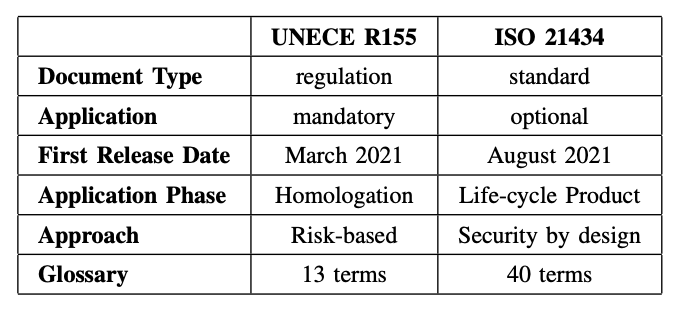
\includegraphics[width=0.7\linewidth]{figures/diff-standards}
    \caption{Comparison of ISO/SAE 21434 and UNECE WP.29 R155}
    \footnotesize{From \cite{comparison-standard} }
    \label{fig:comparison}
\end{figure}

The development of UNECE R155 and ISO/SAE 21434 arose from the need to enhance cybersecurity in road vehicles to ensure user safety and protect personal data.
Although UNECE R155 was released in March 2021 and ISO/SAE 21434 followed in August 2021, the two documents serve different purposes within the automotive cybersecurity landscape.
Here’s a detailed analysis of their similarities, differences, and limitations.

\subsubsection{Correlations}\label{subsubsec:correlations}

Overall, the UNECE regulations emphasize a comprehensive and systematic approach to cybersecurity in the automotive sector, requiring OEMs to be proactive in identifying risks and implementing suitable mitigations.
ISO 26262 emphasizes the relationship between safety and cybersecurity, ensuring that both aspects are addressed in vehicle design.
UNECE WP.29 R155, instead, provides a legal framework for cybersecurity in vehicles, complementing ISO/SAE 21434 by outlining regulatory requirements and compliance timelines.

\subsubsection{Similarities}

\begin{enumerate}
    \item \textbf{Objectives}: Both UNECE R155 and ISO/SAE 21434 aim to improve cybersecurity throughout the product lifecycle of road vehicles.
    \item \textbf{High-Level Solutions}: Both documents propose high-level solutions and do not prescribe specific implementations, allowing manufacturer flexibility to adopt suitable measures for their contexts.
    \item \textbf{Threat Identification}: UNECE R155 identifies possible threats while ISO/SAE 21434 cites similar scenarios requiring analysis and mitigation.
    \item \textbf{Structured Organization}: Both documents require a structured approach to managing cybersecurity, including
    \item \textbf{CSMS}: Cybersecurity Management Systems and risk identification.
    \item \textbf{Risk Mitigation}: Both emphasize risk mitigation processes, where UNECE R155 focuses on risk management and ISO/SAE 21434 outline specific risk treatment options.
    \item \textbf{Documentation for Compliance}: Documentation required for ISO/SAE 21434 can support compliance with UNECE R155, facilitating a cohesive approach.
    \item \textbf{Continuous Review}: Both standards require continuous monitoring and improvement of cybersecurity measures to address evolving threats.
    \item \textbf{Cost Considerations}: Both UNECE R155 and ISO/SAE 21434 acknowledge the need for cybersecurity compliance that balances implementation costs with operational feasibility.
\end{enumerate}

\subsubsection{Differences}

\begin{enumerate}
    \item \textbf{Type}:
    \begin{enumerate}
        \item \textbf{UNECE R155}: A legally binding regulation that mandates compliance for all UNECE member countries.
        \item \textbf{ISO/SAE 21434}: A non-mandatory standard expected to be widely accepted within the automotive industry.
    \end{enumerate}

    \item \textbf{Timeline}:
    \begin{enumerate}
        \item \textbf{UNECE R155}: Compliance from July 2022 and for all vehicles by July 2024.
        \item \textbf{ISO/SAE 21434}: Became applicable from August 2021.
    \end{enumerate}

    \item \textbf{Application Phases}:
    \begin{enumerate}
        \item \textbf{UNECE R155}: Focused primarily on the homogenization process of new vehicles.
        \item \textbf{ISO/SAE 21434}: Product lifecycle, requiring ongoing documentation for annual audits, from design to decommissioning.
    \end{enumerate}

    \item \textbf{Threat and Mitigation}:
    \begin{enumerate}
        \item \textbf{UNECE R155}: Provides tables outlining specific threats and recommended mitigations.
        \item \textbf{ISO/SAE 21434}: Does not directly address attacks but emphasizes vulnerability analysis and risk assessments.
    \end{enumerate}

    \item \textbf{Compliance Requirements}:
    \begin{enumerate}
        \item \textbf{UNECE R155}: Offers a less detailed list of compliance documentation compared to ISO/SAE 21434.
        \item \textbf{ISO/SAE 21434}: Details the attack feasibility ratings and their implications.
    \end{enumerate}

    \item \textbf{Regulatory Authority}:
    \begin{enumerate}
        \item \textbf{UNECE R155}: Enforced by regulatory authorities in UNECE member states, with compliance being mandatory.
        \item \textbf{ISO/SAE 21434}: Lacks mandatory enforcement, relying on industry acceptance and best practices.
    \end{enumerate}
\end{enumerate}

\subsubsection{Conclusion}\label{subsubsec:conclusion2}

In conclusion, while UNECE R155 and ISO/SAE 21434 share common goals of enhancing cybersecurity in the automotive industry, they differ significantly in their nature, application, and requirements.
UNECE R155 is a binding regulation focused on approval, while ISO/SAE 21434 serves as a comprehensive standard for the entire vehicle lifecycle.
Their complementary nature allows manufacturers to leverage the documentation and processes of one to meet the requirements of the other,
fostering a more robust approach to cybersecurity in road vehicles\cite{comparison-standard}.
The problem remains that the lack of mandatory enforcement in ISO/SAE 21434 could lead to inconsistent implementation across the industry and hinder the standard's effectiveness.